\documentclass[a4j] {jarticle}

    \usepackage[dvipdfmx]{graphicx}
    \usepackage[ top=25truemm,bottom=25truemm,left=25truemm,right=25truemm]
    {geometry}
    \usepackage{ascmac}
    \usepackage{amssymb, amsmath}
    \usepackage{array}
    \usepackage{here}
    \usepackage{plistings}
    \usepackage{listings}
    \usepackage{url}
    \renewcommand{\lstlistingname}{リスト}
    \let\oldenumerate\enumerate
  \renewcommand{\enumerate}{
  \oldenumerate
  \setlength{\itemsep}{1.2pt}
  \setlength{\parskip}{0pt}
  \setlength{\parsep}{0pt}
  }
    \lstset{
      basicstyle={\ttfamily},
      identifierstyle={\small},
      commentstyle={\smallitshape},
      keywordstyle={\small\bfseries},
      ndkeywordstyle={\small},
      stringstyle={\small\ttfamily},
      frame={tb},
      breaklines=true,
      columns=[l]{fullflexible},
      numbers=left,
      xrightmargin=0zw,
      xleftmargin=3zw,
      numberstyle={\scriptsize},
      stepnumber=1,
      numbersep=1zw,
      lineskip=-0.5ex
}

\makeatletter
\def\@thesis{アルゴリズムとデータ構造 レポート}
\def\id#1{\def\@id{#1}}
\def\department#1{\def\@department{#1}}

\def\@maketitle{
\begin{center}
{\huge \@thesis \par} %修士論文と記載される部分
\vspace{10mm}
{\LARGE\bf \@title \par}% 論文のタイトル部分
\vspace{10mm}
{\Large \@date\par}	% 提出年月日部分
\vspace{20mm}
{\Large \@department \par}	% 所属部分
{\Large 学籍番号 \@id \par}	% 学籍番号部分
\vspace{10mm}
{\Large 氏名 \@author}% 氏名 
\end{center}
\par\vskip 1.5em
}

\makeatother

\title{多倍長演算}
\date{提出日 令和2年2月3日}
\department{組番号 407}
\id{17406}
\author{金澤雄大}


    \begin{document}
    \maketitle
    \thispagestyle{empty}
    \clearpage
    \addtocounter{page}{-1}

\section{計算内容}
    授業で作成した多倍長演算のプログラムを用いて,ゼータ関数$\zeta(s)$の$s=4$の場合から$\pi$を1000桁程度計算する.しかし,
    1000桁を求めるには非常に時間がかかるため,時間が許す限り可能な桁を求めることにする.

\subsection{開発環境}
開発環境を表\ref{kankyou}に示す.
\begin{table}[H]
  \caption{開発環境}
  \label{kankyou}
  \begin{center}
      \begin{tabular}{l|l}\hline
        CPU & Intel Core i7-6500 2.50Ghz\\
        メモリ & 16.0GB DDR3 \\
        OS & Windows 10 Pro \\
        コンパイラ & GCC 7.4.0 \\
        \hline
      \end{tabular}
  \end{center}
  \end{table}

\section{プログラムの説明}
本章では計算に用いた定数,および構造体,および関数の説明に述べる.
\subsection{NUMBER構造体と定数}
多倍長変数の桁数KETAと基数RADIXをオブジェクト形式マクロで定義する.桁数は多倍長演算を行うときに必要な桁数を設定する.
基数は10000とする.\\
 多倍長変数をNUMBER構造体として定義する.各桁の値を保存するint型の配列nと,多倍長変数の符号(正,または負)
を表すint型の変数signを構造体のメンバとする.多倍長変数の配列は長さがKETAで,RADIXを10000としているので
各要素が0~9999までの値を保持する.配列のi番目の要素を$a_i$と書くことにすると,多倍長変数の配列は$a_0$が0~1000の位であり,
$a_{KETA-1}$が最上位桁である.多倍長変数の符号は表\ref{sign}に示すように,$1$のとき正,$-1$のとき負として扱う.
多倍長変数の値が$0$のとき符号が正であることに注意する必要がある.$-0$と$+0$を混同して扱うとエラーの原因になるから,
本プログラムでは一律して$+0$で扱う.
\begin{table}[H]
  \caption{符号変数の値と多倍長変数の値の符号}
  \label{sign}
  \begin{center}
      \begin{tabular}{|l|l|}\hline
        符号変数の値 & 多倍長変数の値の符号\\ \hline
      \hline
      1 & 正または0 \\ \hline
      -1 & 負 \\ \hline
      \end{tabular}
  \end{center}
  \end{table}

  リスト\ref{const_st}に桁数KETA,基数RADIX,およびNUMBER構造体のプログラムを示す.
  リスト\ref{const_st}では桁数KETAを150桁,基数RADIXを10000と定義している.また
  多倍長変数としてNUMBER構造体を定義している.
  \begin{lstlisting}[basicstyle=\ttfamily\footnotesize, frame=single,label=const_st,caption=定数とNUMBER構造体のソースコード]
#define KETA 150 //桁数
#define RADIX 10000 //基数
struct NUMBER{
    int n[KETA];
    int sign;
};
  \end{lstlisting}

  
\subsection{isZero関数}
  多倍長変数が$0$であることを確認する関数としてisZero関数を作成する.
  表\ref{isZero}にisZero関数の機能,および引数,および返り値を示す.isZero関数では
  第一引数で渡された多倍長変数aが$0$であるかを確認し,$0$であれば$0$を返す.aが$0$でないときは$-1$を返す.
  \begin{table}[H]
    \caption{isZero関数の概要}
    \label{isZero}
    \begin{center}
        \begin{tabular}{|l|l|}\hline
        機能 & 多倍長変数が0であるかを調べる関数.\\ \hline
        引数 & struct NUMBER *a\\ \hline
        返り値の型 & int\\ \hline
        返り値 & 多倍長変数aが0のとき0,0でなければ-1\\ \hline
        \end{tabular}
    \end{center}
    \end{table}

    リスト\ref{iszero_pro}にisZero関数のソースコードを示す.isZero関数の内部ではリスト\ref{iszero_pro}の4~8行目
    に示すようにfor文を用いて多倍長変数の配列を1桁ずつ0であることを確認している.0でない桁が1つでも
    見つかればその時点でfor文から脱出し,-1を返す.全ての桁が0であれば0を返す.
    \begin{lstlisting}[basicstyle=\ttfamily\footnotesize, frame=single,label=iszero_pro,caption=isZero関数のソースコード]
//aが0かをチェック
//0->return 0 else->return -1 
int isZero(struct NUMBER *a){
    int i;
    for(i=0; i<KETA; i++){
        if(a->n[i]!=0){
            return -1;
        }
    }
    return 0;
}
    \end{lstlisting}
\subsection{setSign関数}
  多倍長変数に符号をセットする関数としてsetSign関数を作成する.直接符号を設定することができるが,セッターを用いる
  ことで符号がおかしな値(例えば999,-1234)に設定されるのを防ぐことができる.
表\ref{setSign}にsetSign関数の機能,および引数,および返り値を示す.第一引数で与えた多倍長変数aの符号を
第二引数で与えた符号変数sの値に対応する多倍長変数の符号に設定することでsetSign関数の機能を実現する.
\begin{table}[H]
  \caption{setSign関数の概要}
  \label{setSign}
  \begin{center}
      \begin{tabular}{|l|l|}\hline
      機能 & 多倍長変数の符号を設定する関数.\\ \hline
      引数 & struct NUMBER *a,int s\\ \hline
      返り値の型 & int\\ \hline
      返り値 & 成功(0),失敗(-1).\\ \hline
      \end{tabular}
  \end{center}
  \end{table}

  リスト\ref{set_pro}にsetSign関数のソースコードを示す.setSign関数の内部では最初に,第一引数の多倍長変数が
  0であるか確認する.もしaが0で負にセットしようとしているとき,$-0$が作成されてしまうのでエラーとして$-1$を返して
  処理を終了する.リスト\ref{set_pro}では5~8行目がこの処理にあたる部分である.次に$s$の値によって場合分けをして符号をセットする処理を行う.$s=1$のときaの符号を正に,$s=-1$のときaの符号を負
  にセットして処理を終了する.$s$がその他の値であるときエラーとして$-1$を返して処理を終了する.リスト\ref{set_pro}では10~18行目がこの処理にあたる部分である.
  \begin{lstlisting}[basicstyle=\ttfamily\footnotesize, frame=single,label=set_pro,caption=setSign関数のソースコード]
//aに符号をセット 
//aが0のときに-をセットしようとするとreturn -1
int setSign(struct NUMBER *a,int s){

    if((isZero(a)==0)&&(s==-1)){
        printf("aは0です\n");
        return -1;
    }

    if(s==1){
        a->sign = 1;
        return 0;
    }else if(s==-1){
        a->sign = -1;
        return 0;
    }else{
        return -1;
    }
}    
  \end{lstlisting}


\subsection{getSign関数}
多倍長変数の符号を取り出す関数としてgetSign関数を作成する.setSign関数同様にゲッターを設けることで
おかしな入力が混入し,符号に異常が発生することを防ぐ.
表\ref{getSign}にgetSign関数の機能,および引数,および返り値を示す.
getSign関数は第一引数で渡された多倍長変数の符号をint型の返り値によって取得する関数である.
\begin{table}[H]
  \caption{getSign関数の概要}
  \label{getSign}
  \begin{center}
      \begin{tabular}{|l|l|}\hline
      機能 & 多倍長変数の符号を取得する関数.\\ \hline
      引数 & struct NUMBER *a\\ \hline
      返り値の型 & int\\ \hline
      返り値 & aが正または0(1),aが負(-1).\\ \hline
      \end{tabular}
  \end{center}
  \end{table}

  リスト\ref{getsign_pro}にgetSign関数のソースコードを示す.getSign関数の内部では多倍長変数aの符号変数$s$
  を返す処理を行っている.
  \begin{lstlisting}[basicstyle=\ttfamily\footnotesize, frame=single,label=getsign_pro,caption=getSign関数のソースコード]
//aの符号を取得
int getSign(struct NUMBER *a){
    if(a->sign==1){
        return 1;
    }else{
        return -1;
    }
}
  \end{lstlisting}
\subsection{clearByZero関数}
  多倍長変数をゼロクリアする関数としてclearByZero関数を作成する.
表\ref{clearByZero}にclearByZero関数の機能,および引数,および返り値を示す.
表\ref{clearByZero}に示すようにclearByZero関数は第一引数で渡す多倍長変数をゼロクリアする.
失敗することはないと仮定して,返り値はvoidとする.
\begin{table}[H]
  \caption{clearByZero関数の概要}
  \label{clearByZero}
  \begin{center}
      \begin{tabular}{|l|l|}\hline
      機能 & 多倍長変数をゼロクリアし,符号を正に設定する関数.\\ \hline
      引数 & struct NUMBER *a\\ \hline
      返り値の型 & void\\ \hline
      返り値 & -\\ \hline
      \end{tabular}
  \end{center}
  \end{table}

  リスト\ref{clr}にclearByZero関数のソースコードを示す.clearByZero関数の内部では,最初にfor文を用いて
  多倍長変数の値を保存している配列の要素に0を代入している(リスト\ref{clr}の5~7行目).
  次にsetSign関数を用いて符号を正に設定して処理を終了している.

  \begin{lstlisting}[basicstyle=\ttfamily\footnotesize, frame=single,label=clr,caption=clearByZero関数のソースコード]
//aをゼロクリア
void clearByZero(struct NUMBER *a){
    int i;

    for(i=0; i<KETA;i++){
        a->n[i] = 0;
    }

    setSign(a,1);
}
  \end{lstlisting}

\subsection{getKeta関数}
多倍長変数の桁数を取得する関数として,getKeta関数を作成する.
表\ref{getKeta}にgetKeta関数の機能,および引数,および返り値を示す.
getKeta関数は第一引数で渡された多倍長変数の桁数を返り値とする関数である.
\begin{table}[H]
  \caption{getKeta関数の概要}
  \label{getKeta}
  \begin{center}
      \begin{tabular}{|l|l|}\hline
      機能 & 多倍長変数の桁数を取得する関数.\\ \hline
      引数 & struct NUMBER *a\\ \hline
      返り値の型 & int\\ \hline
      返り値 & 多倍長変数aの桁数.\\ \hline
      \end{tabular}
  \end{center}
  \end{table}

  リスト\ref{getketa_pro}にgetKeta関数のソースコードを示す.getKeta関数の内部では,最初に
  配列の最上位から1桁ずつ0でない桁を探す.0でない桁が見つからない場合はaが0桁であるので0を返す.
  0でない桁が見つかった場合について説明する.i桁で0でない桁を見つけたとする.0でない桁の値は1,2,3,4桁のいずれかである.この
  桁数をtとすると全体の桁数は$i\times 4 -(4-t)$桁であるからこの値を返す.リスト\ref{getketa_pro}のソースコードでは
  $4-t$をjとして求めている.

  \begin{lstlisting}[basicstyle=\ttfamily\footnotesize, frame=single,label=getketa_pro,caption=getKeta関数のソースコード]
// aの桁数を返す
int getKeta(struct NUMBER *a){
    int i,j,base,temp,acopy;
    base = RADIX/10;
    for(i=KETA-1; i>=0; i--){
        if(a->n[i]!=0){
            //printf("a->n[%d] = %4d\n",i,a->n[i]);
            acopy=a->n[i];
            for(j=0;j<(int)log10(RADIX);j++){
                temp = acopy/base;
                acopy %= base;
                if(temp!=0){
                    //printf("j = %d\n",j);
                    return (i+1)*(int)log10(RADIX)-j;
                }
                base/=10;
            }
        }
    }
    return 0;
}
  \end{lstlisting}
\subsection{dispNumber関数}
多倍長変数の符号と値を表示するdispNumber関数を作成する.
表\ref{dispNumber}にdispNumber関数の機能,および引数,および返り値を示す.
dispNumber関数は,第一引数で渡された多倍長変数の符号($+$,$-$のいずれか)と値を表示する関数である.
\begin{table}[H]
  \caption{dispNumber関数の概要}
  \label{dispNumber}
  \begin{center}
      \begin{tabular}{|l|l|}\hline
      機能 & 多倍長変数の符号および各桁の値を表示する.\\ \hline
      引数 & struct NUMBER *a\\ \hline
      返り値の型 & void\\ \hline
      返り値 & -\\ \hline
      \end{tabular}
  \end{center}
  \end{table}

  リスト\ref{disp_pro}にdispNumber関数のソースコードを示す.dispNumber関数の内部では,最初に
  getSign関数で多倍長変数の符号を取得し,表示する.次にリスト\ref{disp_pro}の11~13行目に示すように,
  多倍長変数の値を上位桁$a_{KETA-1}$から順番に$a_0$まで表示している.
  \begin{lstlisting}[basicstyle=\ttfamily\footnotesize, frame=single,label=disp_pro,caption=dispNumber関数のソースコード]
// aを全桁表示
void dispNumber(struct NUMBER *a){
    int i;

    if(getSign(a)==1){
        printf("+ ");
    }else{
        printf("- ");
    }

    for(i=KETA-1; i>=0; i--){
        printf("%04d ",a->n[i]);
    }
}
  \end{lstlisting}
\subsection{dispNumberZeroSuppress関数}
桁数の大きい多倍長変数を表示するときに上位桁の0を省略したい.この操作をゼロサプレスという.そこで上位桁の0を省略して
多倍長変数の符号と値を表示するdispNumberZeroSuppress関数を作成する.
表\ref{dispNumberZeroSuppress}にdispNumberZeroSuppress関数の機能,および引数,および返り値を示す.
表示方法がdispNumber関数と異なるだけであるから,引数および返り値はdispNumber関数と同じである.
\begin{table}[H]
  \caption{dispNumberZeroSuppress関数の概要}
  \label{dispNumberZeroSuppress}
  \begin{center}
      \begin{tabular}{|l|l|}\hline
      機能 & 多倍長変数の符号および各桁の値を上位桁の0を省略して表示する.\\ \hline
      引数 & struct NUMBER *a\\ \hline
      返り値の型 & void\\ \hline
      返り値 & -\\ \hline
      \end{tabular}
  \end{center}
  \end{table}

  リスト\ref{dispZ_pro}にdispNumberZeroSuppress関数のソースコードを示す.dispNumberZeroSuppress関数の
  内部では最初に,getSign関数を用いて符号を取得し表示する.次にリスト\ref{dispZ_pro}の12~14行目に示すように
  ゼロサプレスを行う多倍長変数aが0であるときに画面出力が行われないことを防ぐため,isZero関数を用いてaが0かを
  判別し,0であれば0と表示して終了する.0でなければ配列の要素上位桁から一桁ずつ0でないか確認し,0であるときは
  画面に出力しない.0ではない数が現れて以降は,全ての桁を表示する処理を行う(リスト\ref{dispZ_pro}の15~24行目).
  \begin{lstlisting}[basicstyle=\ttfamily\footnotesize, frame=single,label=dispZ_pro,caption=dispNumberZeroSuppress関数のソースコード]
// aを全桁表示(ゼロサプレス)
void dispNumberZeroSuppress(struct NUMBER *a){
    int i;
    int j=1;

    if(getSign(a)==1){
        printf("+ ");
    }else{
        printf("- ");
    }

    if(isZero(a)==0){
        printf("0");
    }
    for(i=KETA-1; i>=0; i--){
        if(j){
            if(a->n[i] != 0){
                printf("%d ",a->n[i]);
                j=0;
            }
        }else{
        printf("%04d ",a->n[i]);
        }
    }
}
  \end{lstlisting}
\subsection{copyNumber関数}
多倍長変数を別の多倍長変数にコピーする関数として,copyNumber関数を作成する.
表\ref{copyNumber}にcopyNumber関数の機能,および引数,および返り値を示す.
copyNumber関数は第一引数の多倍長変数の符号と値を別の多倍長変数にコピーする関数である.
\begin{table}[H]
  \caption{copyNumber関数の概要}
  \label{copyNumber}
  \begin{center}
      \begin{tabular}{|l|l|}\hline
      機能 & 多倍長変数の符号と値を別の多倍長変数にコピーする.\\ \hline
      引数 & struct NUMBER *a,struct NUMBER *b\\ \hline
      返り値の型 & void\\ \hline
      返り値 & -\\ \hline
      \end{tabular}
  \end{center}
  \end{table}

  リスト\ref{cp_pro}にcopyNumber関数のソースコードを示す.copyNumber関数の内部では
  bの構造体にaの構造体を渡す処理を行っている.
  \begin{lstlisting}[basicstyle=\ttfamily\footnotesize, frame=single,label=cp_pro,caption=copyNumber関数のソースコード]
//aをbにコピー
void copyNumber(struct NUMBER *a,struct NUMBER *b){
    *b=*a;
}
  \end{lstlisting}
\subsection{getAbs関数}
多倍長変数の絶対値を別の多倍長変数に代入する関数として,getAbs関数を作成する.
表\ref{getAbs}にgetAbs関数の機能,および引数,および返り値を示す.
getAbs関数は第一引数で渡された多倍長変数aの絶対値を第二引数で渡された多倍長変数bに代入する関数である.
\begin{table}[H]
  \caption{getAbs関数の概要}
  \label{getAbs}
  \begin{center}
      \begin{tabular}{|l|l|}\hline
      機能 & 多倍長変数の絶対値を別の多倍長変数に代入する.\\ \hline
      引数 & struct NUMBER *a,struct NUMBER *b\\ \hline
      返り値の型 & void\\ \hline
      返り値 & -\\ \hline
      \end{tabular}
  \end{center}
  \end{table}

  リスト\ref{abs_pro}にgetAbs関数のソースコードを示す.getAbs関数の内部では,最初にcopyNumber関数を用いてaの値をb
  にコピーする.次にsetSign関数を用いてbの符号を正に設定する.
  \begin{lstlisting}[basicstyle=\ttfamily\footnotesize, frame=single,label=abs_pro,caption=getAbs関数のソースコード]
//aの絶対値をbに代入
void getAbs(struct NUMBER *a,struct NUMBER *b){
    copyNumber(a,b);
    setSign(b,1);
}
  \end{lstlisting}

\subsection{mulBy10関数}
多倍長変数の10倍を別の多倍長変数に代入する関数として,mulBy10関数を作成する.
表\ref{mulBy10}にmulBy10関数の機能,および引数,および返り値を示す.mulBy10関数は第一引数の多倍長変数aの10倍を第二引数の多倍長変数bに
代入する関数である.オーバーフローしたときには返り値として-1を返す.
\begin{table}[H]
  \caption{mulBy10関数の概要}
  \label{mulBy10}
  \begin{center}
      \begin{tabular}{|l|l|}\hline
      機能 & 多倍長変数の値を10倍する.\\ \hline
      引数 & struct NUMBER *a,struct NUMBER *b\\ \hline
      返り値の型 & int\\ \hline
      返り値 & 成功(0),失敗(-1)\\ \hline
      \end{tabular}
  \end{center}
  \end{table}

  リスト\ref{mulby10_pro}にmulBy10関数のソースコードを示す.mulBy10関数の内部では,最初に,setSign関数を用いてaの符号をbに設定する.
  次にリスト\ref{mulby10_pro}の6~8行目に示すようにaの最上位桁が0であることを確認する.もし0でなければ10倍したときにオーバーフロー
  してしまうので-1を返す.オーバーフローが起きないことを確認したのでbにaの10倍を代入する処理を行う.
  \begin{lstlisting}[basicstyle=\ttfamily\footnotesize, frame=single,label=mulby10_pro,caption=mulBy10関数のソースコード]
//aを10倍してbに代入
int mulBy10(struct NUMBER *a,struct NUMBER *b){
    int i,temp;
    int carry =0;
    setSign(b,getSign(a));
    if(a->n[KETA-1]/(int)(RADIX/10) != 0){
        return -1;
    }

    b->n[KETA-1] = a->n[KETA-1]*10;
    for(i=KETA-2; i>=0;i--){
        temp = a->n[i]*10;
        carry = temp/RADIX;
        b->n[i] = temp % RADIX;
        b->n[i+1]+=carry;
    }
    return 0;
}
  \end{lstlisting}

\subsection{mulBy10000関数}
多倍長変数の10000倍を別の多倍長変数に代入する関数としてmulBy10000関数を作成する.
表\ref{mulBy10000}にmulBy10000関数の機能,および引数,および返り値を示す.mulBy10000関数は第一引数の多倍長変数aの10000倍を第二引数の多倍長変数bに
代入する関数である.
\begin{table}[H]
  \caption{mulBy10000関数の概要}
  \label{mulBy10000}
  \begin{center}
      \begin{tabular}{|l|l|}\hline
      機能 & 多倍長変数の値を10000倍する.\\ \hline
      引数 & struct NUMBER *a,struct NUMBER *b\\ \hline
      返り値の型 & int\\ \hline
      返り値 & 成功(0),失敗(-1)\\ \hline
      \end{tabular}
  \end{center}
  \end{table}

  リスト\ref{mulby10000_pro}にmulBy10000関数のソースコードを示す.mulBy10000関数の内部では,最初にsetSign関数を用いて
  bにaの符号をセットする.次にリスト\ref{mulby10000_pro}の5~7行目に示すようにaの最上位桁が0であることを確認する.
  最上位桁が0でなければ10000倍したときにオーバーフローしてしまうため-1を返す.オーバーフローが起きないことを確
  認したのでbにaの10000倍を代入する処理を行う.
  \begin{lstlisting}[basicstyle=\ttfamily\footnotesize, frame=single,label=mulby10000_pro,caption=mulBy10000関数のソースコード]
//aを10000倍してbに代入
int mulBy10000(struct NUMBER *a,struct NUMBER *b){
    int i;
    setSign(b,getSign(a));
    if(a->n[KETA-1]!=0){
        return -1;
    }

    for(i=0; i<KETA-1;i++){
        b->n[i+1] = a->n[i];
    }
    b->n[0]=0;
    return 0;
}
  \end{lstlisting}

\subsection{setInt関数}
int型の変数を多倍長変数に変換する関数として,setInt関数を作成する.
表\ref{setInt}にsetInt関数の機能,および引数,および返り値を示す.setInt関数は第二引数のint型の値xを第一引数の多倍長変数a
に代入する関数である.多倍長変数の桁数が足りない場合はint型の変数を変換しきれないので-1を返す.
\begin{table}[H]
  \caption{setInt関数の概要}
  \label{setInt}
  \begin{center}
      \begin{tabular}{|l|l|}\hline
      機能 & int型の変数を多倍長変数に設定する.\\ \hline
      引数 & struct NUMBER *a,int x\\ \hline
      返り値の型 & int\\ \hline
      返り値 & 成功(0),失敗(-1)\\ \hline
      \end{tabular}
  \end{center}
  \end{table}

  setInt関数の処理内容は次の通りである.
  \begin{enumerate}
    \item 多倍長変数の桁数が足りることを確認する.足りない場合は-1をreturnする.
    \item xが負の時xの絶対値を作業用変数(int型)に代入する.
    \item aの下位桁から順にxの作業用変数の値を設定する.
    \item setInt関数を用いてaにxの符号を設定する.
  \end{enumerate}

  リスト\ref{setint_pro}にsetInt関数のソースコードを示す.setInt関数の内部では,最初にリスト\ref{setint_pro}の4~7行目に示すように
多倍長変数の桁数が足りるか確認を行う.足りなければ-1を返して終了する.次にaをゼロクリアして
int型の値xの絶対値をaにセットする.最後にxの符号をsetSign関数を用いてaの符号にセットする.
  \begin{lstlisting}[basicstyle=\ttfamily\footnotesize, frame=single,label=setint_pro,caption=setInt関数のソースコード]
//xをaに代入
int setInt(struct NUMBER *a,int x){
    int temp,i;
    if(KETA<3){
        printf("KETAが足りません\n");
        return -1;
    }

    clearByZero(a);

    temp=x;
    if(x<0){
        temp*=-1;
    }
    for(i=0;i<3;i++){
        a->n[i]=temp%RADIX;
        temp-=a->n[i];
        temp/=RADIX;
    }

    if(x<0){
        setSign(a,-1);
    }else{
        setSign(a,1);
    }
    return 0;
}
\end{lstlisting}
\subsection{numComp関数}
多倍長変数の大小を比較する関数としてnumComp関数を作成する.
表\ref{numComp}にnumComp関数の機能,および引数,および返り値を示す.numComp関数は第一引数の多倍長変数aと第二引数の多倍長変数bの
の大小を比較する関数である.
\begin{table}[H]
  \caption{numComp関数の概要}
  \label{numComp}
  \begin{center}
      \begin{tabular}{|l|l|}\hline
      機能 & 多倍長変数の大小を比較する.\\ \hline
      引数 & struct NUMBER *a,struct NUMBER *b\\ \hline
      返り値の型 & int\\ \hline
      返り値 & a>b(1),a<b(-1),a=b(0),不明なエラー(623)\\ \hline
      \end{tabular}
  \end{center}
  \end{table}
  
  リスト\ref{numcomp_pro}にnumComp関数のソースコードを示す.
\begin{lstlisting}[basicstyle=\ttfamily\footnotesize, frame=single,label=numcomp_pro,caption=numComp関数のソースコード]
//多倍長の大小比較 a==b:0 a>b:1 a<b:-1
int numComp(struct NUMBER *a,struct NUMBER *b){
    int i,Sa,Sb;
    Sa = getSign(a);
    Sb = getSign(b);

    // a+ b-
    if((Sa==1)&&(Sb==-1)){
        return 1;
    }

    //a- b+
    if((Sa==-1)&&(Sb==1)){
        return -1;
    }
    //a+ b+
    if((Sa==1)&&(Sb==1)){
        for(i=KETA-1; i>=0; i--){
            if(a->n[i] > b->n[i]){
                return 1;
            }

            if(a->n[i] < b->n[i]){
                return -1;
            }
        }
        return 0;
    }

    if((Sa==-1)&&(Sb==-1)){
        for(i=KETA-1; i>=0; i--){
            if(a->n[i] > b->n[i]){
                return -1;
            }

            if(a->n[i] < b->n[i]){
                return 1;
            }
        }
        return 0;
    }
    return 623;
}
\end{lstlisting}

numComp関数の処理内容は次の通りである.a,bの符号によって場合わけをして大小を比較する.
  \begin{enumerate}
    \item aおよびbの符号をgetSign関数を用いて取得する.
    \item aが正,bが負のときa>bであるから1をreturnする.
    \item aが負,bが正のときb<aであるから-1をreturnする.
    \item a,bがともに正のとき,最上位桁から順に比較し,大小関係が確定させる.
    \item a,bがともに負のとき,最上位桁から順に比較し,大小関係が確定させる.
  \end{enumerate}

\subsection{add関数}
2つの多倍長変数の和を計算する関数として,add関数を作成する.
表\ref{add}にadd関数の機能,および引数,および返り値を示す.add関数は第一引数の多倍長変数aと第二引数の多倍長変数bの
和$a+b$を計算し,第三引数の多倍長変数$c$に計算結果を代入する関数である.$a+b$の計算結果がオーバーフローしたときには
cをゼロクリアして終了する.関数の返り値は関数の実行が正常に行われたか検知するために使用する.
\begin{table}[H]
  \caption{add関数の概要}
  \label{add}
  \begin{center}
      \begin{tabular}{|l|l|}\hline
      機能 & a+bを計算し,cに計算結果を代入する.\\ \hline
      引数 & struct NUMBER *a,struct NUMBER *b,struct NUMBER *c\\ \hline
      返り値の型 & int\\ \hline
      返り値 & 成功(0),失敗(-1),不明なエラー(623)\\ \hline
      \end{tabular}
  \end{center}
  \end{table}

  リスト\ref{add}にadd関数のソースコードを示す.
  \begin{lstlisting}[basicstyle=\ttfamily\footnotesize, frame=single,label=add_pro,caption=add関数のソースコード]
// c<- a+b
int add(struct NUMBER *a,struct NUMBER *b,struct NUMBER *c){
    int Sa = getSign(a);
    int Sb = getSign(b);
    struct NUMBER Nd,Ne;
    int d,i;
    int e=0;
    //a+ b+
    if((Sa==1)&&(Sb==1)){
        for(i=0;i<KETA;i++){
            d = a->n[i] + b->n[i] +e;
            c->n[i] = d%RADIX;
            e = (d - c->n[i]) /RADIX;
        }
        if(e==1){
            clearByZero(c);
            return -1;
        }
        setSign(c,1);
        return 0;
        }
    
        //a+ b-
    if((Sa==1)&&(Sb==-1)){
        getAbs(b,&Nd);
        sub(a,&Nd,c);
        return 0;
    }

    //a- b+
    if((Sa==-1)&&(Sb==1)){
        getAbs(a,&Nd);
        sub(b,&Nd,c);
        return 0;
    }

    //a- b-
    if((Sa==-1)&&(Sb==-1)){
        getAbs(a,&Nd);
        getAbs(b,&Ne);
        add(&Nd,&Ne,c);
        setSign(c,-1);
        return 0;
    }
    return 623; //不明なエラー検出
}
  \end{lstlisting}

  add関数の処理内容について説明する.
  add関数はa,bの符号によって処理が異なる.a,bがともに正のとき次の手順で計算する.この手順は授業中に紹介された
  筆算の方法である.
  \begin{enumerate}
    \item i(int型),およびe(int型)を0にセットする.
    \item aのi桁目$a_i$を取り出す.
    \item bのi桁目$b_o$を取り出す.
    \item dに$a_i+b_i+e$を代入する.
    \item dの1~1000の位の値を取り出してcのi桁目にセットする.
    \item dの10000の位を取り出してeに代入する.
    \item iをインクリメントする.i$\leqq$ KETA-1のとき,手順2に戻る.
    \item eが0でない場合オーバーフローであるのでclearByZero関数を用いてcをゼロクリアして終了する.
    \item cの符号をsetSign関数を用いて正にセットし終了する.
  \end{enumerate}

  次にaが正,bが負の場合を考える.この場合$a+b$は式(\ref{aba1})に示すように変形できるから,
  aとbの絶対値をとった値を減算関数(sub関数)に渡す処理をしている.ただし,sub関数については次節で実装している.
  \begin{equation}
  c = a+b = a- |b|
  \label{aba1}
  \end{equation}

  aが負,bが正の場合を考える.この場合$a+b$は式(\ref{aba2})に示すように変形できるから
  bとaの絶対値をとった値をsub関数に渡す処理をしている.
  \begin{equation}
  c = a+b = b- |a|
  \label{aba2}
  \end{equation}

  a,bがともに負のときを考える.この場合$a+b$は式(\ref{aba3})に示すように変形できるから,
  再度add関数を呼び出しaの絶対値を取った値と,bの絶対値を取った値を渡し,計算結果
  の符号を負に設定する処理をしている.
  \begin{equation}
    c = a+b = - (|a|+|b|)
    \label{aba3}
    \end{equation}

\subsection{sub関数}
2つの多倍長変数の差を計算する関数として,sub関数を作成する.
表\ref{sub}にsub関数の機能,および引数,および返り値を示す.sub関数は第一引数の多倍長変数aと第二引数の多倍長変数bの
差$a-b$を計算し,第三引数の多倍長変数$c$に計算結果を代入する関数である.$a-b$の計算結果がオーバーフローしたときには
cをゼロクリアして終了する.関数の返り値は関数の実行が正常に行われたか検知するために使用する.
\begin{table}[H]
  \caption{sub関数の概要}
  \label{sub}
  \begin{center}
      \begin{tabular}{|l|l|}\hline
      機能 & a-bを計算し,cに計算結果を代入する.\\ \hline
      引数 & struct NUMBER *a,struct NUMBER *b,struct NUMBER *c\\ \hline
      返り値の型 & int\\ \hline
      返り値 & 成功(0),失敗(-1),不明なエラー(623)\\ \hline
      \end{tabular}
  \end{center}
  \end{table}

  \begin{lstlisting}[basicstyle=\ttfamily\footnotesize, frame=single,label=sub_pro,caption=sub関数のソースコード]
// c<- a-b 
int sub(struct NUMBER *a,struct NUMBER *b,struct NUMBER *c){
    struct NUMBER Nd,Ne;
    int Sa = getSign(a);
    int Sb = getSign(b);
    int i;
    int h=0;
    //a+ b+
    if((Sa==1)&&(Sb==1)){
    if(numComp(a,b)==1){
        setSign(c,1);
        for(i=0;i<KETA;i++){
            a->n[i]-=h;
            if(a->n[i]>=b->n[i]){
                c->n[i] = a->n[i] - b->n[i];
                h=0;
            }else{
                c->n[i] = RADIX + a->n[i] - b->n[i];
                h=1;
            }
        }
        return 0;
    }

    if(numComp(a,b)==-1){
        for(i=0;i<KETA;i++){
            b->n[i]-=h;
            if(b->n[i]>=a->n[i]){
                c->n[i] = b->n[i] - a->n[i];
                h=0;
            }else{
                c->n[i] = RADIX
                 + b->n[i] - a->n[i];
                h=1;
            }
        }
        setSign(c,-1);
    }

    if(numComp(a,b)==0){
        clearByZero(c);
    }
    return 0;
    }

    //a+ b-
    if((Sa==1)&&(Sb==-1)){
        getAbs(b,&Nd);
        add(a,&Nd,c);
        return 0;
    }

    //a- b+
    if((Sa==-1)&&(Sb==1)){
        getAbs(a,&Nd);
        add(&Nd,b,c);
        setSign(c,-1);
        return 0;
    }

    //a- b-
    if((Sa==-1)&&(Sb==-1)){
        getAbs(b,&Ne);
        add(a,&Ne,c);
        return 0;
    }

    return 623;//不明なエラー検出
}
  \end{lstlisting}
  sub関数の内部処理を説明する.
  sub関数はa,bの符号と大小関係によって処理が異なる.a$\geqq$bかつ両方が正のとき次の手順で計算する.
  a$<$bのとき式(\ref{abs1})のように変形できるので再度sub関数を呼び出して$b-a$を計算し,計算結果に負の符号を設定する.
  \begin{enumerate}
    \item i(int型),およびh(int型)を0にセットする.
    \item aのi桁目$a_i$を取り出す.
    \item bのi桁目$b_i$を取り出す.
    \item $a_i$からhを引く.
    \item $a_i$$\geq$$b_i$であれば$c_i=a_i-b_i$を計算し,h=0とする.
    \item $a_i<b_i$であれば$c_i=10000+a_i-b_i$を計算し,h=1とする.
    \item iをインクリメントする.i$\leqq$KETA-1のとき2に戻る.
    \item hが1のときオーバーフローであるからclearByZero関数を用いてcをゼロクリアし,終了する.
    \item setSign関数を用いてcの符号を正にセットして終了する.
  \end{enumerate}

  \begin{equation}
    c = a-b = -(b-a)
    \label{abs1}
    \end{equation}

    次にaが正,bが負の場合を考える.この場合$a-b$は式(\ref{abs2})に示すように変形できるから,
  aとbの絶対値をとった値の和をadd関数で計算する.
  \begin{equation}
    c = a-b = a + |b|
    \label{abs2}
    \end{equation}

    aが負,bが正の場合を考える.この場合$a-b$は式(\ref{abs3})に示すように変形できるから,
  bとaの絶対値をとった値の和をadd関数で計算し符号を負にセットする.
  \begin{equation}
    c = a-b = -(|a| + b)
    \label{abs3}
    \end{equation}

    aがbがともに負の場合を考える.この場合$a-b$は式(\ref{abs4})に示すように変形できるから,
  aとbの絶対値をとった値の和をadd関数で計算する.
  \begin{equation}
    c = a-b = a + |b|
    \label{abs4}
    \end{equation}

\subsection{increment関数}
多倍長変数にインクリメントを行う関数としてincrement関数を作成する.インクリメントとは変数の値を1増やす演算のことである.
表\ref{increment}にincrement関数の機能,および引数,および返り値を示す.increment関数は第一引数の多倍長変数の値aをインクリメントし,
第二引数の多倍長変数bに代入する関数である.オーバーフローが起きたときには-1を返す.
\begin{table}[H]
  \caption{increment関数の概要}
  \label{increment}
  \begin{center}
      \begin{tabular}{|l|l|}\hline
      機能 & 多倍長変数をインクリメントする.\\ \hline
      引数 & struct NUMBER *a,struct NUMBER *b\\ \hline
      返り値の型 & int\\ \hline
      返り値 & 成功(0),失敗(-1)\\ \hline
      \end{tabular}
  \end{center}
  \end{table}

  リスト\ref{increment_pro}にincrement関数のソースコードを示す.increment関数の内部では,
  最初に作業用の多倍長変数oneにsetInt関数を用いて1を代入する.次にadd関数を用いて$a+1$を計算しbに代入する.
  オーバーフローが起きたとき,add関数は表\ref{add}より返り値として成功(0),失敗($-1$)を返すので,これをincrement関数の返り値
  としている.
  \begin{lstlisting}[basicstyle=\ttfamily\footnotesize, frame=single,label=increment_pro,caption=increment関数のソースコード]
// b<- a++
int increment(struct NUMBER *a,struct NUMBER *b){
    struct NUMBER one;
    int r;
    setInt(&one,1);
    r = add(a,&one,b);
    return r;
}
\end{lstlisting}


\subsection{multiple関数}
2つの多倍長変数の積を計算する関数としてmultiple関数を作成する.
表\ref{multiple}にmultiple関数の機能,および引数,および返り値を示す.multiple関数は第一引数の多倍長変数aと
第二引数の多倍長変数bの積を計算し,第三引数の多倍長変数cに代入する関数である.オーバーフローが起きたとき,返り値として$-1$を返す.
\begin{table}[H]
  \caption{multiple関数の概要}
  \label{multiple}
  \begin{center}
      \begin{tabular}{|l|l|}\hline
      機能 & a$\times$bを計算しcに代入する.\\ \hline
      引数 & struct NUMBER *a,struct NUMBER *b,struct NUMBER *c\\ \hline
      返り値の型 & int\\ \hline
      返り値 & 成功(0),失敗(-1)\\ \hline
      \end{tabular}
  \end{center}
  \end{table}

  リスト\ref{multiple_pro}にmultiple関数のソースコードを示す.
  \begin{lstlisting}[basicstyle=\ttfamily\footnotesize, frame=single,label=multiple_pro,caption=multiple関数のソースコード]
// c<-a*b
int multiple(struct NUMBER *a,struct NUMBER *b,struct NUMBER *c){
    int e,h,i,j;
    int Sa = getSign(a);
    int Sb = getSign(b);
    struct NUMBER d,d2,ee;
    clearByZero(c);

    if(Sa==1 && Sb==1){
        for(i=0;i<KETA;i++){
            h=0;
            clearByZero(&d);
            for(j=0;j<KETA;j++){
                e=(a->n[j]* b->n[i])+h;
                d.n[j] = e%RADIX;
                e-=d.n[j];
                h = e/RADIX;
            }
            if(h != 0){
                clearByZero(c);
                return -1;
            }

            for(j=0;j<i*((int)log10(RADIX));j++){
                if(mulBy10(&d,&d2)==-1){
                    clearByZero(c);
                    return -1;
                }
                copyNumber(&d2,&d);
            }

            if(add(c,&d,c)==-1){
                clearByZero(c);
                return -1;
            }
        }
        return 0;
    }

    if(Sa==-1 && Sb==1){
        getAbs(a,&d);
        i = multiple(&d,b,c);
        if(i==-1){
            return -1;
        }
        setSign(c,-1);
        return 0;
    }

    if(Sa==1 && Sb==-1){
        getAbs(b,&d);
        i = multiple(a,&d,c);
        if(i==-1){
            return -1;
        }
        setSign(c,-1);
        return 0;
    }
    if(Sa==-1 && Sb ==-1){
        getAbs(a,&d);
        getAbs(b,&ee);
        i = multiple(&d,&ee,c);
        if(i==-1){
            return -1;
        }
        setSign(c,1);
        return 0;
    }
    return 623;
}
  \end{lstlisting}

  multiple関数の内部処理を説明する.
  multiple関数の処理はaおよびbの符号によって場合分けを行う.a,bがともに正のときの処理内容は次の通りである.
  \begin{enumerate}
    \item cをゼロクリアする.
    \item i$=$0(int型)とする.
    \item bのi桁目$b_i$を取り出す.
    \item 作業用の変数として,h(int型)および多倍長変数dをゼロクリアする.
    \item j$=$0(int型)とする.
    \item aのj桁目$a_j$を取り出す.
    \item 作業用の変数e(int型)に$a_j\times b_i+h$を代入する.
    \item eの1000の位まで取り出し,$d_j$に代入する.
    \item eの10000の位を取り出しhに代入する.
    \item j$=$KETA-1のとき手順11を行う.hが0でない場合,オーバーフローである.
    \item jをインクリメントして手順5に戻る.
    \item mulBy10関数を用いてdを$10^i$倍する.ここでもオーバーフローが起こりえるので検出する.
    \item cにdを加える.ここでもオーバーフローが起こりえる.
    \item i$=$KETA-1のときループ終了する.
    \item iをインクリメントし手順3に戻る.
  \end{enumerate}
  aが正,bが負のとき$a\times b$は式(\ref{abm2})に示すように書き直せるから,
  再度multiple関数を呼び出し,aとbの絶対値をとった値を渡せばよい.符号はsetSign関数を用いて負に設定する.
  \begin{equation}
    c = a\times b = -(a\times |b|)
    \label{abm2}
    \end{equation}

    aが負,bが正のとき$a\times b$は式(\ref{abm3})に示すように書き直せるから,
  再度multiple関数を呼び出し,aの絶対値をとった値とbを渡せばよい.符号はsetSign関数を用いて負に設定する.
  \begin{equation}
    c = a\times b = -(|a|\times b)
    \label{abm3}
    \end{equation}

    a,bがともに負のとき$a\times b$は式(\ref{abm4})に示すように書き直せるから,
  再度multiple関数を呼び出し,aの絶対値をとった値とbの絶対値を渡せばよい.符号はsetSign関数を用いて正に設定する.
  \begin{equation}
    c = a\times b = (|a|\times |b|)
    \label{abm4}
    \end{equation}

\subsection{divide\_2関数}
多倍長変数の割り算を行う関数としてdivide\_2関数を作成する.
表\ref{divide_2}にdivide\_2関数の機能,および引数,および返り値を示す.divide\_2関数は第一引数の多倍長変数の値a,第二引数b,
第三引数c,第四引数bとすると$a\div b$を計算し,計算結果の商をc,剰余をdに代入する関数である.
\begin{table}[H]
  \caption{divide\_2関数の概要}
  \label{divide_2}
  \begin{center}
      \begin{tabular}{|l|l|}\hline
      機能 & a$\div$bを計算する,\\ \hline
      引数 & struct NUMBER *a,struct NUMBER *b,struct NUMBER *c,struct NUMBER *d\\ \hline
      返り値の型 & int\\ \hline
      返り値 & 成功(0),失敗(-1)\\ \hline
      \end{tabular}
  \end{center}
  \end{table}

リスト\ref{divide_2_pro}にdivide\_2関数のソースコードを示す.
  \begin{lstlisting}[basicstyle=\ttfamily\footnotesize, frame=single,label=divide_2_pro,caption=divide\_2関数のソースコード]
//割り算高速化
// a/b = c...d
int divide_2(struct NUMBER *a,struct NUMBER *b,struct NUMBER *c,struct NUMBER *d){
    struct NUMBER n,p,q,r;
    int over;
    int Sa = getSign(a);
    int Sb = getSign(b);
    clearByZero(c);
    clearByZero(d);

    if(isZero(b)==0){
        printf("div by 0\n");
        return -1;
    }

    copyNumber(a,&n);

    if(Sa==1 && Sb==1){
        while(1){
            if(numComp(&n,b)==-1){
                break;
            }
            copyNumber(b,&p);
            setInt(&q,1);
            while(1){
                over = mulBy10(&p,&r);
               if(over == -1){
                    break;
                }
                if(numComp(&n,&r)==-1){
                    break;
                }
                copyNumber(&r,&p);
                mulBy10(&q,&r);
                copyNumber(&r,&q);
            }
            sub(&n,&p,&r);
            copyNumber(&r,&n);
            add(c,&q,&r);
            copyNumber(&r,c);

        }
        copyNumber(&n,d);
        return 0;
    }
    if(Sa==1 && Sb==-1){
        getAbs(b,&p);
        divide_2(&n,&p,c,d);
        setSign(c,-1);
        return 0;
    }

    if(Sa==-1 && Sb==1){
        getAbs(a,&p);
        divide_2(&p,b,c,d);
        setSign(c,-1);
        setSign(d,-1);
        return 0;
    }

    if(Sa==-1 && Sb==-1){
        getAbs(a,&p);
        getAbs(b,&q);
        divide_2(&p,&q,c,d);
        setSign(d,-1);
        return 0;
    }
    return 623;
}
  \end{lstlisting}
  divide\_2関数の内部処理について説明する.
  divide\_2関数の処理内容はaおよびbの符号によって異なる.aおよびbがともに正のときの処理内容を次に示す.
  最初に0除算が発生していないことを確認してから除算処理を行っている.

  \begin{enumerate}
    \item bが0でないことを確認する.0であれば終了する.
    \item cをゼロクリアする.
    \item numComp関数を用いてaとbの大小を調べる.a$<$bであれば手順11に飛ぶ.
    \item dにbを代入する.
    \item 作業用の多倍長変数pに1をセットする.
    \item dを10倍する操作を繰り返して,a$>$dを満たす最大のdを見つける.
    \item 手順6でdを10倍したのと同じ回数だけeを10倍する.
    \item aからdを引く.
    \item cにeを足す.
    \item 手順3に戻る.
    \item dにaをコピーして終了する.
    \end{enumerate}

    aが正,bが負のとき,$a\div b$の商cは負,剰余dは正の値になるから,再度divide\_2関数を呼び出して
    aとbの絶対値を渡し,計算結果の商を負の値にセットする.aが負,bが正のとき,$a\div b$の商cは負
    ,剰余dは負の値になるから,再度divide\_2関数を呼び出してaの絶対値とbを渡し,計算結果の商と剰余を負の値にセットする.
    a,bがともに負のとき,$a\div b$の商cは正,剰余dは負の値になるから,再度divide\_2関数を呼び出してaの絶対値とbの絶対値を渡し,
    計算結果の商と剰余を負の値にセットする.

\subsection{sqrt\_newton関数}
多倍長変数の平方根を計算する関数としてsqrt\_newton関数を作成する.
表\ref{sqrt_newton}にsqrt\_newton関数の機能,および引数,および返り値を示す.sqrt\_newton関数はNewton-Raphson法を用いて第一引数の多倍長変数aの平方根を
計算し,第二引数の多倍長変数bに代入する.
\begin{table}[H]
  \caption{sqrt\_newton関数の概要}
  \label{sqrt_newton}
  \begin{center}
      \begin{tabular}{|l|l|}\hline
      機能 & 多倍長変数の平方根を計算する.\\ \hline
      引数 & struct NUMBER *a,struct NUMBER *b\\ \hline
      返り値の型 & int\\ \hline
      返り値 & 成功(0),失敗(-1)\\ \hline
      \end{tabular}
  \end{center}
  \end{table}

  Newton-Raphson法とは方程式$f(x)=0$を反復的に解く方法である.解を$s=\alpha$,$f(x)$の一階微分を$f'(x)$,適当な初期値を$x_0$とする.
  式(\ref{nr1})を$x_1$,$x_2$...と反復計算を行うことで$x$の近似値$x_i$が真の値$\alpha$に近づいていく.
  \begin{equation}
    x_{i+1} = x_i - \frac{f(x_i)}{f'(x_i)}
    \label{nr1}
    \end{equation}
  
    Newton-Raphson法を用いて$N$の平方根を計算するために$f(x)$を式(\ref{nr2})のように設定する.
    \begin{equation}
      f(x) = x^2 -N
      \label{nr2}
      \end{equation}

      $f(x)$の一階微分は式(\ref{nr3})であるから,反復計算に式(\ref{nr4})を用いればよいことが分かる.
      \begin{equation}
        f(x) = 2x
        \label{nr3}
        \end{equation}

        \begin{eqnarray}
          x_{i+1} &=& x_i - \frac{x_i^2 -N}{2x_i}\\
          &=& \frac{x_i}{2} + \frac{N}{2x_i}\\
          &=& \frac{1}{2} \left( x_i + \frac{N}{x_i} \right)
          \label{nr4}
        \end{eqnarray}

リスト\ref{sqrt_newton_pro}にsqrt\_newton関数のソースコードを示す.
        \begin{lstlisting}[basicstyle=\ttfamily\footnotesize, frame=single,label=sqrt_newton_pro,caption=sqrt\_newton関数のソースコード]
// b<- sqrt{a} (Newton-Raphson法)
int sqrt_newton(struct NUMBER *a,struct NUMBER *b){
    struct NUMBER x,temp,temp2,c,d;
    
    setInt(&d,2);
    divide_2(a,&d,&x,&c);
    if(isZero(&x)==0){
        copyNumber(a,b);
        return 0;
    }

    if(getSign(&x)==-1){
        return -1;
    }

    copyNumber(&x,&d);

    while(1){
        copyNumber(&d,&c);
        copyNumber(&x,&d);

        divide_2(a,&d,&temp,&temp2);
        add(&d,&temp,&temp2);
        setInt(b,2);
        divide_2(&temp2,b,&x,&temp);

        if(numComp(&x,&d)==0){
            break;
        }
        if(numComp(&x,&c)==0){
            if(numComp(&d,&x)==-1){
                copyNumber(&d,&x);
            }
        }   
    }
    copyNumber(&x,b);
    return 0;
}
        \end{lstlisting}
  sqrt\_newton関数の処理内容は次の通りである.
  \begin{enumerate}
    \item 作業用変数xに初期値($\frac{a}{2}$)を代入する.
    \item x=0,または1のとき$\sqrt{a}=a$であるからbにaをコピーして終了する.
    \item xが負の時エラーで-1を返す
    \item 式(\ref{nr4})を反復的に計算する.
    \item 収束,振動を判定する.$k$回目の計算結果が$k-1$回目,または$k-2$回目の計算結果と同じであれば終了する.
  \end{enumerate}

\subsection{zeta4関数}
zeta4関数はゼータ関数$\zeta(s)$の$s=4$のときの値から円周率$\pi$を計算する関数である.
$\zeta(s)$は$s=4$のとき式(\ref{zeta41})である.
\begin{eqnarray}
  \zeta(4) = \sum_{n=1}^{\infty} \frac{1}{n^4} = \frac{\pi^4}{90}
  \label{zeta41}
\end{eqnarray}

手持ちの関数では小数を扱うことができないので$10^\alpha$($\alpha>0$)をかけて式(\ref{zeta10})を
計算する.また無限回ループを繰り返すことができないのでb回ループを繰り返した時の近似値を求める.
\begin{eqnarray}
  10^\alpha \sum_{n=1}^{b} \frac{1}{n^4} = \frac{10^\alpha \times \pi^4}{90}
  \label{zeta10}
\end{eqnarray}

表\ref{zeta4}にzeta4関数の機能,および引数,および返り値を示す.zeta4関数では第一引数で受け取った
多倍長変数aに計算結果(円周率)を代入する.第二引数のloopは式(\ref{zeta10})における
bのことである.第三引数のketaは式(\ref{zeta10})の$\alpha$のことである.
第四引数のdispは途中経過を何桁おきに表示するかを格納する変数である.
\begin{table}[H]
  \caption{zeta4関数の概要}
  \label{zeta4}
  \begin{center}
      \begin{tabular}{|l|l|}\hline
      機能 & 円周率を計算する.\\ \hline
      引数 & struct NUMBER *a,int loop,int keta,int disp\\ \hline
      返り値の型 & int\\ \hline
      返り値 & 成功(0),失敗(-1)\\ \hline
      \end{tabular}
  \end{center}
  \end{table}

リスト\ref{zeta4_pro}にzeta4関数のソースコードを示す
  \begin{lstlisting}[basicstyle=\ttfamily\footnotesize, frame=single,label=zeta4_pro,caption=zeta4関数のソースコード]
//zeta(4)から円周率を計算
//結果をaに代入
// int loop 反復回数
// int keta r/n^4のrの値
// int disp 途中経過の表示回数
int zeta4(struct NUMBER *a,int loop,int keta,int disp){

    if(loop<=0){
        printf("loopが不正な値です.\n");
        return -1;
    }

    if(keta>KETA*(int)log10(RADIX) || keta<=0){
        printf("ketaが不正な値です.\n");
        return -1;
    }
    if(disp>loop || disp<=0){
        printf("loopが不正な値です.\n");
        return -1;
    }

    int i,r;
    struct NUMBER n,b,temp,temp2,tenE;

    clearByZero(&b);
    setInt(&tenE,1);
    for(i=0;i<keta/(int)log10(RADIX);i++){
        r = mulBy10000(&tenE,&temp);
        copyNumber(&temp,&tenE);
    }

    for(i=0;i<keta%(int)log10(RADIX);i++){
        r = mulBy10(&tenE,&temp);
        copyNumber(&temp,&tenE);
    }

    i=1;
    gettimeofday(&tv,NULL);
    tstart =(double)tv.tv_sec + (double)tv.tv_usec *1.e-6;

    printf("多倍長桁数KETA = %d\n",KETA);
    printf("loop回数 = %d\n",loop);
    printf("keta = %d\n",keta);
    printf("途中経過表示 %d 回毎\n\n",disp);
    printf("----- start loop -----\n");
    while(1){
        //iをセット
        setInt(&n,i);   
        //i^4を計算
        r = multiple(&n,&n,&temp);
        if(r==-1){
            printf("overflow in n^2\n");
            return -1;
        }
        multiple(&temp,&temp,&n);
        if(r==-1){
            printf("overflow in n^4\n");
            return -1;
        }

        divide_2(&tenE,&n,&temp,&temp2);
        add(&b,&temp,&temp2);
        copyNumber(&temp2,&b);

        if(i%disp==0){
            printf("pi^4/90[i = %d] = ",i);
            dispNumberZeroSuppress(&b);
            printf("\n\n");
            gettimeofday(&tv,NULL);
            tend =(double)tv.tv_sec + (double)tv.tv_usec *1.e-6;
            printf("所要時間 = %f秒\n\n",tend-tstart);
        }
        if(i==loop){
            break;
        }
        i++;
    }
    printf("----- finish loop -----\n");
    printf("pi^4/90 = ");
    dispNumberZeroSuppress(&b);
    printf("\n\n");
    
    setInt(&temp2,90);
    multiple(&b,&temp2,&temp);
    printf("pi^4 = ");
    dispNumberZeroSuppress(&temp);
    printf("\n\n");

    //平方根を取るために桁調整
    copyNumber(&temp,&temp2);
    r = getKeta(&temp2)%(int)log10(RADIX);
    if(r!=4){
        for(i=0;i<r; i++){
            mulBy10(&temp2,&temp);
            copyNumber(&temp,&temp2);
        }
    }

    // 平方根をとってpi^2を計算
    //printf("平方根1回目直前桁数 : %d\n",getKeta(&temp2));
    printf("----- calculate pi^2 -----\n");
    sqrt_newton(&temp2,&temp);
    printf("pi^2 = ");
    dispNumberZeroSuppress(&temp);
    printf("\n\n");

    //平方根を取るために桁調整
    copyNumber(&temp,&temp2);
    r = getKeta(&temp2)%2;
    if(r==0){
        mulBy10(&temp2,&temp);
        copyNumber(&temp,&temp2);
    }

    // 平方根をとってpiを計算
    //printf("平方根2回目直前桁数 : %d\n",getKeta(&temp2));
    printf("----- calculate pi -----\n");
    sqrt_newton(&temp,&temp2);
    /*printf("pi = ");
    dispNumberZeroSuppress(&temp2);
    printf("\n");*/

    gettimeofday(&tv,NULL);
    tend =(double)tv.tv_sec + (double)tv.tv_usec *1.e-6;
    printf("所要時間 = %f秒\n\n",tend-tstart);

    copyNumber(&temp2,a);
    return 0;
}
  \end{lstlisting}
zeta4関数の処理内容を次に示す.zeta4関数はこれまでに作成した関数を下請けとして円周率を計算する関数である.
\begin{enumerate}
  \item $\frac{1}{n^4}$の和を多倍長変数bに代入するのでbをゼロクリアしておく.
  \item $10^\alpha$を作業用多倍長変数tenEに代入する.
  \item i=1(int型)を用意する.
  \item setInt関数を用いて作業用多倍長変数nにiを代入する.
  \item $n^2$を作業用多倍長変数tempに代入する.
  \item $temp^2$を作業用多倍長変数nに代入する.これで$n^4$を計算できた.
  \item $tenE \div n$を計算し作業用多倍長変数temp2に代入する.
  \item $i \div disp$の剰余が0であれば途中経過を表示する.
  \item iとloop回数が等しければ手順11に飛ぶ.
  \item iをインクリメントして手順4に戻る.
  \item temp2を90倍してtempに代入する.これで$\pi^4$を計算できた.
  \item 平方根を取るために桁調整を行う.
  \item sqrt\_newton関数を用いて$\pi^2$を計算する.
  \item 平方根を取るために桁調整を行う.
  \item sqrt\_newton関数を用いて$\pi$を計算する.
\end{enumerate}
\subsection{fileNumberZeroSuppress関数}
円周率の計算結果をファイルに書き込む関数としてfileNumberZeroSuppress関数を作成する.
表\ref{fileNumberZeroSuppress}にfileNumberZeroSuppress関数の機能,および引数,および返り値を示す.
fileNumberZeroSuppress関数はdispNumberZeroSuppress関数をファイル書き込みに変更したものである.
第一引数の多倍長変数aをゼロサプレスしてcalpi.txtに書き込む.計算によってもとめた
円周率を書き込むための関数であり,符号が負の多倍長変数には対応していない.
\begin{table}[H]
  \caption{fileNumberZeroSuppress関数の概要}
  \label{fileNumberZeroSuppress}
  \begin{center}
      \begin{tabular}{|l|l|}\hline
      機能 & 多倍長変数をファイルに書き込む.\\ \hline
      引数 & struct NUMBER *a\\ \hline
      返り値の型 & int\\ \hline
      返り値 & 成功(0),失敗(-1)\\ \hline
      \end{tabular}
  \end{center}
  \end{table}

  リスト\ref{fileNumberZeroSuppress_pro}にfileNumberZeroSuppress関数のソースコードを示す.
  fileNumberZeroSuppress関数の内部では最初に,ローカル変数として書き込みを行うファイル名を文字列として定義する.
  次にfopen関数を用いて書き込みモードでファイルを開く.何らかの理由でファイルが開けなかった場合は,処理を終了する.
  ファイルを開くと,aの値をゼロサプレスしてファイルに書き込みを行う.
  \begin{lstlisting}[basicstyle=\ttfamily\footnotesize, frame=single,label=fileNumberZeroSuppress_pro,caption=fileNumberZeroSuppress関数のソースコード]
//aをファイルに書き込み
int fileNumberZeroSuppress(struct NUMBER *a){
    char *fname = "calpi.txt";
    FILE *fp;
    int i;
    int j=1;
    if((fp = fopen(fname,"w"))==NULL){
        printf("ファイルを開けませんでした\n");
        return -1;
    }else{
        printf("\nresult write in %s ...",fname);
        if(isZero(a)==0){
        printf("0");
    }
    for(i=KETA-1; i>=0; i--){
        if(j){
            if(a->n[i] != 0){
                fprintf(fp,"%d",a->n[i]);
                j=0;
            }
        }else{
        fprintf(fp,"%04d",a->n[i]);
        }
    }
    printf("complete\n");
    fclose(fp);
    }
    return 0;
}
\end{lstlisting}
\subsection{calcheck関数}
計算によって求めた円周率と真の円周率の値を比較し,一致した桁数を表示する関数としてcalcheck関数を
作成する.表\ref{calcheck}にcalcheck関数の機能,および引数,および返り値を示す.calcheck関数は計算によって求めた
円周率と真の値を比較し,小数点以下の一致桁数を表示する関数である.

\begin{table}[H]
  \caption{calcheck関数の概要}
  \label{calcheck}
  \begin{center}
      \begin{tabular}{|l|l|}\hline
      機能 & 計算による円周率と真の値を比較する.\\ \hline
      引数 & void\\ \hline
      返り値の型 & int\\ \hline
      返り値 & 成功(0),失敗(-1)\\ \hline
      \end{tabular}
  \end{center}
  \end{table}

  リスト\ref{calcheck_pro}calcheck関数の処理内容を説明する.事前に計算によって求めた円周率をfileNumberZeroSuppress関数を用いて
  calpi.txtに書き込む.さらに,Wolfarm Alpha\cite{key2}から円周率1000桁をコピーしてpi.txtに書き込む.リスト\ref{pi_real}にpi.txtの冒頭100文字を示す.
  ただしどちらのファイルについても浮動小数点を削除しておく.calpi.txtとpi.txtを値が一致しなくなるまで1文字ずつ読み込み,小数点以下の一致桁を表示する.
  \begin{lstlisting}[basicstyle=\ttfamily\footnotesize, frame=single,label=calcheck_pro,caption=calcheck関数のソースコード]
//pi.txtとcalpi.txtを比較
int calcheck(void){
    char *fname1 = "pi.txt";
    char *fname2 = "calpi.txt";
    FILE *fp1;
    FILE *fp2;
    int ch1;
    int ch2;
    int i=0;

    if((fp1 = fopen(fname1,"r"))==NULL){
        printf("ファイル %s を開けませんでした\n",fname1);
        return -1;
    }else{
        if((fp2 = fopen(fname2,"r"))==NULL){
        printf("ファイル %s を開けませんでした\n",fname2);
        return -1;
        }else{
            while (( ch2 = fgetc(fp2)) != EOF ) {
                ch1 = fgetc(fp1);
            //putchar(ch2);
            //putchar(ch1);
            if(ch1!=ch2){
                break;
            }
            i++;
    }
    printf("\n小数点以下 %d 桁一致\n",i-1);
    fclose(fp2);
    fclose(fp1);
    }
    }
    return 0;
}
  \end{lstlisting}

  \begin{lstlisting}[basicstyle=\ttfamily\footnotesize, frame=single,label=pi_real,caption=pi.txtの内容]
31415926535897932384626433832795028841971693993751
05820974944592307816406286208998628034825342117067
  \end{lstlisting}

\subsection{メイン関数}
メイン関数を作成する.リスト\ref{main_pro}にメイン関数のソースコードを示す.メイン関数では,最初に多倍長変数piを定義する.zeta4関数にpiを渡して円周率を計算する.
zeta4関数で計算に失敗した場合はメイン関数を終了する.
zeta4関数が失敗していなければ,piには円周率の計算結果が入っているから,dispNumberZeroSuppress関数にpiを渡して
ファイルに計算結果を書き込む.最後に計算結果の精度の確認を行う.calcheck関数を用いて小数点以下の一致桁数を確認して
メイン関数を終了する.
\begin{lstlisting}[basicstyle=\ttfamily\footnotesize, frame=single,label=main_pro,caption=メイン関数のソースコード]
#include<stdio.h>
#include "mulprec.h"

#define calpi

int main(void){
    #ifdef calpi    
    struct NUMBER pi;
    int loop = 1000; //ループ回数
    int keta = 130;
    int disp =100; //disp回おきに途中経過を表示
    int r;
    r = zeta4(&pi,loop,keta,disp);
    if(r==0){
        printf("\n----- result -----\n");
        printf("pi = ");
        dispNumberZeroSuppress(&pi);
        printf("\n");
    //結果をファイルに書き込み
    fileNumberZeroSuppress(&pi);
    //検算
    printf("\n----- 検算 -----\n");
    calcheck();
    }else{
        printf("zata4関数を異常終了しました\n");
    }
    #endif

    return 0;
}
\end{lstlisting}

    
\section{実行結果}
    本章では短時間で計算を行ったときの実行結果,および長時間で計算を行ったときの実行結果について述べる.
    \subsection{短時間で計算を行ったときの実行結果}
    作成した関数が正常に動作しているか確認するために,次の条件で実行を行った.
    \begin{itemize}
        \item 桁数KETA$=150$
        \item ループ回数loop$=1000$
        \item 割り算を行うために10倍する回数keta$=130$
        \item 途中経過の表示回数disp$=100$
      \end{itemize}
      実行結果を図\ref{r1}に示す.図\ref{r1}のresultと書いてある上の所要時間296.7秒から処理時間はおおよそ5分であることが読み取れる.
      また,resultの項目から円周率の計算結果が$pi=3.1415...$であることが読み取れる.さらに,検算の項目から検算の結果小数点以下9桁が
      真の円周率の値と一致していることが分かる.

      \begin{figure}[H]
        \centering
        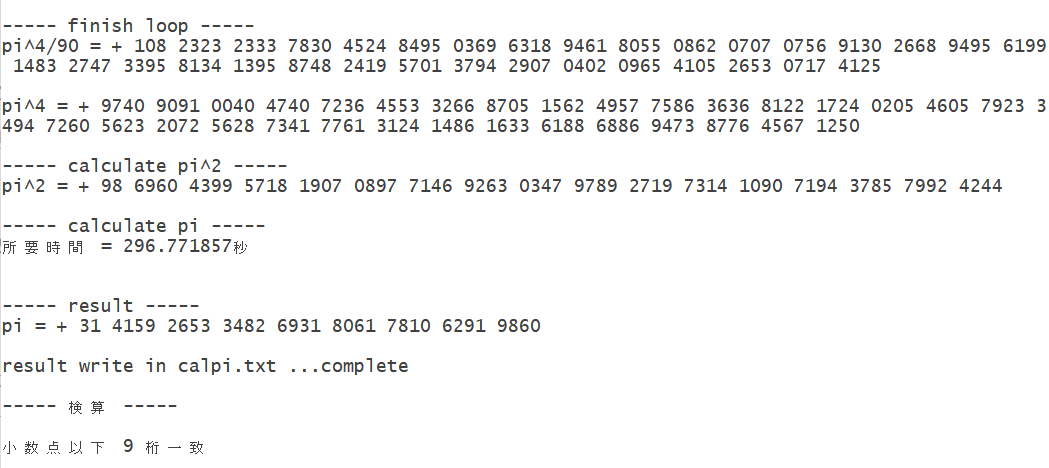
\includegraphics[scale=0.8]{result1.png}
        \caption{ループ回数を少なくして実行した結果}
       \label{r1}
      \end{figure}


      \subsection{長時間で計算を行ったときの実行結果}
      短時間で計算を実行した結果,円周率の計算プログラムが正常に動くことが確かめられたから,次の条件で実行を行った.
    \begin{itemize}
        \item 桁数KETA$=150$
        \item ループ回数loop$=500000$
        \item 割り算を行うために10倍する回数keta$=120$
        \item 途中経過の表示回数disp$=1000$
      \end{itemize}

      実行結果を図\ref{r2}に示す.ループ回数を500000回にしたとき,処理に85874.9秒かかったことが読み取れる.
      時間に直すと23時間51分14.9秒である.また,円周率の計算結果は小数点以下17桁一致していることが読み取れる.

      \begin{figure}[H]
        \centering
        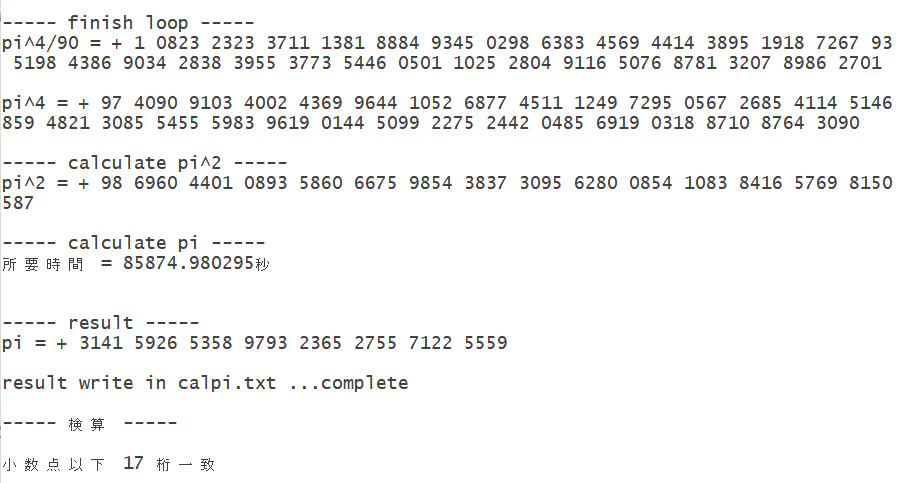
\includegraphics[scale=0.82]{result2.png}
        \caption{ループ回数を増やして実行した結果}
       \label{r2}
      \end{figure}

    \section{考察}
    2つの実行結果だけでは明らかにデータ不足であるから桁数を固定し,ループ回数を変化させたときの
    円周率の精度(小数点以下)および実行時間の変化を測定した.ループ回数以外の条件を次に示す.
    \begin{itemize}
        \item 桁数KETA$=150$
        \item 割り算を行うために10倍する回数keta$=120$
        \item 途中経過の表示回数disp$=100$
      \end{itemize}

    図\ref{loop_seido}にループ回数と精度の関係を示す.
    図\ref{loop_seido}はループ回数(底が10の対数)と小数点以下の円周率の計算の精度を表している.
    図\ref{loop_seido}から精度はループ回数の対数に比例することが読み取れる.このことから収束が非常に遅い
    ことが分かる.最小二乗法を用いて円周率を小数点以下1000桁求める
    ために必要なループ回数を計算すると,おおよそ$10^{43000}$であることが分かった.これは現実的なループ回数の数値ではない.
    このことからゼータ関数$\zeta(s)$が$s=4$のときのアルゴリズムで円周率を1000桁求めることは現実的ではないと
    考えられる.
    \begin{figure}[H]
        \centering
        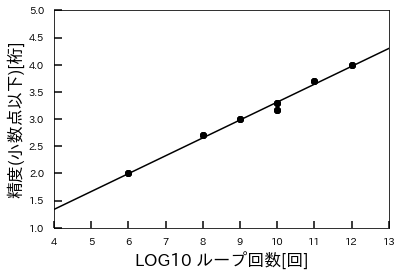
\includegraphics[scale=0.6]{loop_seido.png}
        \caption{ループ回数と精度の関係}
       \label{loop_seido}
      \end{figure}

      図\ref{loop_time}にループ回数と時間の関係を示す.図\ref{loop_time}から,
      時間はループ回数に比例することが読み取れる.最小二乗法を用いてループが1増えたときの
      処理時間を計算すると,5.9秒でることが分かった.円周率を1000桁求めるためには,$10^{43000}$
      回ループを回す必要があるのでこれに5.9秒をかけると現実的な時間ではないことが分かる.
      このことからもゼータ関数$\zeta(s)$が$s=4$のときのアルゴリズムで円周率を1000桁求めることは現実的ではないと
    考えられる.
      \begin{figure}[H]
        \centering
        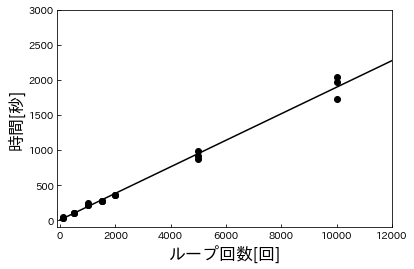
\includegraphics[scale=0.6]{loop_time.png}
        \caption{ループ回数と時間の関係}
       \label{loop_time}
      \end{figure}

    \section{プログラムリスト}
    mulprec.cのプログラムをリスト\ref{mulprec}に示す.ただし,授業で作成したプログラムの基数を10000に変更している.
    \begin{lstlisting}[basicstyle=\ttfamily\footnotesize, frame=single,label=mulprec,caption=mulprec.cのソースコード]
#include<stdio.h>
#include<stdlib.h>
#include<sys/time.h>
#include<math.h>
#include<limits.h>      

#define KETA 150 //桁数
#define RADIX 10000 //基数

struct timeval tv;
double tstart,tend;

struct NUMBER{
    int n[KETA];
    int sign;
};

//aが0かをチェック
//0->return 0 else->return -1 
int isZero(struct NUMBER *a){
    int i;
    for(i=0; i<KETA; i++){
        if(a->n[i]!=0){
            return -1;
        }
    }
    return 0;
}

// aの桁数を返す
int getKeta(struct NUMBER *a){
    int i,j,base,temp,acopy;
    base = RADIX/10;
    for(i=KETA-1; i>=0; i--){
        if(a->n[i]!=0){
            //printf("a->n[%d] = %4d\n",i,a->n[i]);
            acopy=a->n[i];
            for(j=0;j<(int)log10(RADIX);j++){
                temp = acopy/base;
                acopy %= base;
                if(temp!=0){
                    //printf("j = %d\n",j);
                    return (i+1)*(int)log10(RADIX)-j;
                }
                base/=10;
            }
        }
    }
    return 0;
}

//aに符号をセット 
//aが0のときに-をセットしようとするとreturn -1
int setSign(struct NUMBER *a,int s){

    if((isZero(a)==0)&&(s==-1)){
        printf("aは0です\n");
        return -1;
    }

    if(s==1){
        a->sign = 1;
        return 0;
    }else if(s==-1){
        a->sign = -1;
        return 0;
    }else{
        return -1;
    }
}

//aの符号を取得
int getSign(struct NUMBER *a){
    if(a->sign==1){
        return 1;
    }else{
        return -1;
    }
}



//aをゼロクリア
void clearByZero(struct NUMBER *a){
    int i;

    for(i=0; i<KETA;i++){
        a->n[i] = 0;
    }

    setSign(a,1);
}


// aを全桁表示
void dispNumber(struct NUMBER *a){
    int i;

    if(getSign(a)==1){
        printf("+ ");
    }else{
        printf("- ");
    }

    for(i=KETA-1; i>=0; i--){
        printf("%04d ",a->n[i]);
    }
}


// aを全桁表示(ゼロサプレス)
void dispNumberZeroSuppress(struct NUMBER *a){
    int i;
    int j=1;

    if(getSign(a)==1){
        printf("+ ");
    }else{
        printf("- ");
    }

    if(isZero(a)==0){
        printf("0");
    }
    for(i=KETA-1; i>=0; i--){
        if(j){
            if(a->n[i] != 0){
                printf("%d ",a->n[i]);
                j=0;
            }
        }else{
        printf("%04d ",a->n[i]);
        }
    }
}

//下位k桁に乱数を生成
void setRnd(struct NUMBER *a,int k){
    int i;
    clearByZero(a);

    for(i=0; i<k; i++){
        a->n[i] = random()%(RADIX);
    }
    if(random()%2==1){
        setSign(a,1);
    }else{
        setSign(a,-1);
    }
}

//aをbにコピー
void copyNumber(struct NUMBER *a,struct NUMBER *b){
    *b=*a;
}

//aの絶対値をbに代入
void getAbs(struct NUMBER *a,struct NUMBER *b){
    copyNumber(a,b);
    setSign(b,1);
}

//aを10倍してbに代入
int mulBy10(struct NUMBER *a,struct NUMBER *b){
    int i,temp;
    int carry =0;
    setSign(b,getSign(a));
    if(a->n[KETA-1]/(int)(RADIX/10) != 0){
        return -1;
    }

    b->n[KETA-1] = a->n[KETA-1]*10;
    for(i=KETA-2; i>=0;i--){
        temp = a->n[i]*10;
        carry = temp/RADIX;
        b->n[i] = temp % RADIX;
        b->n[i+1]+=carry;
    }
    return 0;
}

//aを10000倍してbに代入
int mulBy10000(struct NUMBER *a,struct NUMBER *b){
    int i;
    setSign(b,getSign(a));
    if(a->n[KETA-1]!=0){
        return -1;
    }

    for(i=0; i<KETA-1;i++){
        b->n[i+1] = a->n[i];
    }
    b->n[0]=0;
    return 0;
}

//xをaに代入
int setInt(struct NUMBER *a,int x){
    int temp,i;
    if(KETA<3){
        printf("KETAが足りません\n");
        return -1;
    }

    clearByZero(a);

    temp=x;
    if(x<0){
        temp*=-1;
    }
    for(i=0;i<3;i++){
        a->n[i]=temp%RADIX;
        temp-=a->n[i];
        temp/=RADIX;
    }

    if(x<0){
        setSign(a,-1);
    }else{
        setSign(a,1);
    }
    return 0;
}

//多倍長の大小比較 a==b:0 a>b:1 a<b:-1
int numComp(struct NUMBER *a,struct NUMBER *b){
    int i,Sa,Sb;
    Sa = getSign(a);
    Sb = getSign(b);

    // a+ b-
    if((Sa==1)&&(Sb==-1)){
        return 1;
    }

    //a- b+
    if((Sa==-1)&&(Sb==1)){
        return -1;
    }
    //a+ b+
    if((Sa==1)&&(Sb==1)){
        for(i=KETA-1; i>=0; i--){
            if(a->n[i] > b->n[i]){
                return 1;
            }

            if(a->n[i] < b->n[i]){
                return -1;
            }
        }
        return 0;
    }

    if((Sa==-1)&&(Sb==-1)){
        for(i=KETA-1; i>=0; i--){
            if(a->n[i] > b->n[i]){
                return -1;
            }

            if(a->n[i] < b->n[i]){
                return 1;
            }
        }
        return 0;
    }
    return 623;
}

int sub(struct NUMBER *a,struct NUMBER *b,struct NUMBER *c);
// c<- a+b
int add(struct NUMBER *a,struct NUMBER *b,struct NUMBER *c){
    int Sa = getSign(a);
    int Sb = getSign(b);
    struct NUMBER Nd,Ne;
    int d,i;
    int e=0;
    //a+ b+
    if((Sa==1)&&(Sb==1)){
        for(i=0;i<KETA;i++){
            d = a->n[i] + b->n[i] +e;
            c->n[i] = d%RADIX;
            e = (d - c->n[i]) /RADIX;
        }
        if(e==1){
            clearByZero(c);
            return -1;
        }
        setSign(c,1);
        return 0;
        }
    
        //a+ b-
    if((Sa==1)&&(Sb==-1)){
        getAbs(b,&Nd);
        sub(a,&Nd,c);
        return 0;
    }

    //a- b+
    if((Sa==-1)&&(Sb==1)){
        getAbs(a,&Nd);
        sub(b,&Nd,c);
        return 0;
    }

    //a- b-
    if((Sa==-1)&&(Sb==-1)){
        getAbs(a,&Nd);
        getAbs(b,&Ne);
        add(&Nd,&Ne,c);
        setSign(c,-1);
        return 0;
    }
    return 623; //不明なエラー検出
}

// c<- a-b 
int sub(struct NUMBER *a,struct NUMBER *b,struct NUMBER *c){
    struct NUMBER Nd,Ne;
    int Sa = getSign(a);
    int Sb = getSign(b);
    int i;
    int h=0;
    //a+ b+
    if((Sa==1)&&(Sb==1)){
    if(numComp(a,b)==1){
        setSign(c,1);
        for(i=0;i<KETA;i++){
            a->n[i]-=h;
            if(a->n[i]>=b->n[i]){
                c->n[i] = a->n[i] - b->n[i];
                h=0;
            }else{
                c->n[i] = RADIX + a->n[i] - b->n[i];
                h=1;
            }
        }
        return 0;
    }

    if(numComp(a,b)==-1){
        for(i=0;i<KETA;i++){
            b->n[i]-=h;
            if(b->n[i]>=a->n[i]){
                c->n[i] = b->n[i] - a->n[i];
                h=0;
            }else{
                c->n[i] = RADIX
                 + b->n[i] - a->n[i];
                h=1;
            }
        }
        setSign(c,-1);
    }

    if(numComp(a,b)==0){
        clearByZero(c);
    }
    return 0;
    }

    //a+ b-
    if((Sa==1)&&(Sb==-1)){
        getAbs(b,&Nd);
        add(a,&Nd,c);
        return 0;
    }

    //a- b+
    if((Sa==-1)&&(Sb==1)){
        getAbs(a,&Nd);
        add(&Nd,b,c);
        setSign(c,-1);
        return 0;
    }

    //a- b-
    if((Sa==-1)&&(Sb==-1)){
        getAbs(b,&Ne);
        add(a,&Ne,c);
        return 0;
    }

    return 623;//不明なエラー検出
}

// b<- a++
int increment(struct NUMBER *a,struct NUMBER *b){
    struct NUMBER one;
    int r;
    setInt(&one,1);
    r = add(a,&one,b);
    return r;
}

// c<-a*b
int multiple(struct NUMBER *a,struct NUMBER *b,struct NUMBER *c){
    int e,h,i,j;
    int Sa = getSign(a);
    int Sb = getSign(b);
    struct NUMBER d,d2,ee;
    clearByZero(c);

    if(Sa==1 && Sb==1){
        for(i=0;i<KETA;i++){
            h=0;
            clearByZero(&d);
            for(j=0;j<KETA;j++){
                e=(a->n[j]* b->n[i])+h;
                d.n[j] = e%RADIX;
                e-=d.n[j];
                h = e/RADIX;
            }
            if(h != 0){
                clearByZero(c);
                return -1;
            }

            for(j=0;j<i*((int)log10(RADIX));j++){
                if(mulBy10(&d,&d2)==-1){
                    clearByZero(c);
                    return -1;
                }
                copyNumber(&d2,&d);
            }

            if(add(c,&d,c)==-1){
                clearByZero(c);
                return -1;
            }
        }
        return 0;
    }

    if(Sa==-1 && Sb==1){
        getAbs(a,&d);
        i = multiple(&d,b,c);
        if(i==-1){
            return -1;
        }
        setSign(c,-1);
        return 0;
    }

    if(Sa==1 && Sb==-1){
        getAbs(b,&d);
        i = multiple(a,&d,c);
        if(i==-1){
            return -1;
        }
        setSign(c,-1);
        return 0;
    }
    if(Sa==-1 && Sb ==-1){
        getAbs(a,&d);
        getAbs(b,&ee);
        i = multiple(&d,&ee,c);
        if(i==-1){
            return -1;
        }
        setSign(c,1);
        return 0;
    }
    return 623;
}

//割り算高速化
// a/b = c...d
int divide_2(struct NUMBER *a,struct NUMBER *b,struct NUMBER *c,struct NUMBER *d){
    struct NUMBER n,p,q,r;
    int over;
    int Sa = getSign(a);
    int Sb = getSign(b);
    clearByZero(c);
    clearByZero(d);

    if(isZero(b)==0){
        printf("div by 0\n");
        return -1;
    }

    copyNumber(a,&n);

    if(Sa==1 && Sb==1){
        while(1){
            if(numComp(&n,b)==-1){
                break;
            }
            copyNumber(b,&p);
            setInt(&q,1);
            while(1){
                over = mulBy10(&p,&r);
               if(over == -1){
                    break;
                }
                if(numComp(&n,&r)==-1){
                    break;
                }
                copyNumber(&r,&p);
                mulBy10(&q,&r);
                copyNumber(&r,&q);
            }
            sub(&n,&p,&r);
            copyNumber(&r,&n);
            add(c,&q,&r);
            copyNumber(&r,c);

        }
        copyNumber(&n,d);
        return 0;
    }
    if(Sa==1 && Sb==-1){
        getAbs(b,&p);
        divide_2(&n,&p,c,d);
        setSign(c,-1);
        return 0;
    }

    if(Sa==-1 && Sb==1){
        getAbs(a,&p);
        divide_2(&p,b,c,d);
        setSign(c,-1);
        setSign(d,-1);
        return 0;
    }

    if(Sa==-1 && Sb==-1){
        getAbs(a,&p);
        getAbs(b,&q);
        divide_2(&p,&q,c,d);
        setSign(d,-1);
        return 0;
    }
    return 623;
}

// b<- sqrt{a} (Newton-Raphson法)
int sqrt_newton(struct NUMBER *a,struct NUMBER *b){
    struct NUMBER x,temp,temp2,c,d;
    
    setInt(&d,2);
    divide_2(a,&d,&x,&c);
    if(isZero(&x)==0){
        copyNumber(a,b);
        return 0;
    }

    if(getSign(&x)==-1){
        return -1;
    }

    copyNumber(&x,&d);

    while(1){
        copyNumber(&d,&c);
        copyNumber(&x,&d);

        divide_2(a,&d,&temp,&temp2);
        add(&d,&temp,&temp2);
        setInt(b,2);
        divide_2(&temp2,b,&x,&temp);

        if(numComp(&x,&d)==0){
            break;
        }
        if(numComp(&x,&c)==0){
            if(numComp(&d,&x)==-1){
                copyNumber(&d,&x);
            }
        }   
    }
    copyNumber(&x,b);
    return 0;
}

//zeta(4)から円周率を計算
//結果をaに代入
// int loop 反復回数
// int keta r/n^4のrの値
// int disp 途中経過の表示回数
int zeta4(struct NUMBER *a,int loop,int keta,int disp){

    if(loop<=0){
        printf("loopが不正な値です.\n");
        return -1;
    }

    if(keta>KETA*(int)log10(RADIX) || keta<=0){
        printf("ketaが不正な値です.\n");
        return -1;
    }
    if(disp>loop || disp<=0){
        printf("loopが不正な値です.\n");
        return -1;
    }

    int i,r;
    struct NUMBER n,b,temp,temp2,tenE;

    clearByZero(&b);
    setInt(&tenE,1);
    for(i=0;i<keta/(int)log10(RADIX);i++){
        r = mulBy10000(&tenE,&temp);
        copyNumber(&temp,&tenE);
    }

    for(i=0;i<keta%(int)log10(RADIX);i++){
        r = mulBy10(&tenE,&temp);
        copyNumber(&temp,&tenE);
    }

    i=1;
    gettimeofday(&tv,NULL);
    tstart =(double)tv.tv_sec + (double)tv.tv_usec *1.e-6;

    printf("多倍長桁数KETA = %d\n",KETA);
    printf("loop回数 = %d\n",loop);
    printf("keta = %d\n",keta);
    printf("途中経過表示 %d 回毎\n\n",disp);
    printf("----- start loop -----\n");
    while(1){
        //iをセット
        setInt(&n,i);   
        //i^4を計算
        r = multiple(&n,&n,&temp);
        if(r==-1){
            printf("overflow in n^2\n");
            return -1;
        }
        multiple(&temp,&temp,&n);
        if(r==-1){
            printf("overflow in n^4\n");
            return -1;
        }

        divide_2(&tenE,&n,&temp,&temp2);
        add(&b,&temp,&temp2);
        copyNumber(&temp2,&b);

        if(i%disp==0){
            printf("pi^4/90[i = %d] = ",i);
            dispNumberZeroSuppress(&b);
            printf("\n\n");
            gettimeofday(&tv,NULL);
            tend =(double)tv.tv_sec + (double)tv.tv_usec *1.e-6;
            printf("所要時間 = %f秒\n\n",tend-tstart);
        }
        if(i==loop){
            break;
        }
        i++;
    }
    printf("----- finish loop -----\n");
    printf("pi^4/90 = ");
    dispNumberZeroSuppress(&b);
    printf("\n\n");
    
    setInt(&temp2,90);
    multiple(&b,&temp2,&temp);
    printf("pi^4 = ");
    dispNumberZeroSuppress(&temp);
    printf("\n\n");

    //平方根を取るために桁調整
    copyNumber(&temp,&temp2);
    r = getKeta(&temp2)%(int)log10(RADIX);
    if(r!=4){
        for(i=0;i<r; i++){
            mulBy10(&temp2,&temp);
            copyNumber(&temp,&temp2);
        }
    }

    // 平方根をとってpi^2を計算
    //printf("平方根1回目直前桁数 : %d\n",getKeta(&temp2));
    printf("----- calculate pi^2 -----\n");
    sqrt_newton(&temp2,&temp);
    printf("pi^2 = ");
    dispNumberZeroSuppress(&temp);
    printf("\n\n");

    //平方根を取るために桁調整
    copyNumber(&temp,&temp2);
    r = getKeta(&temp2)%2;
    if(r==0){
        mulBy10(&temp2,&temp);
        copyNumber(&temp,&temp2);
    }

    // 平方根をとってpiを計算
    //printf("平方根2回目直前桁数 : %d\n",getKeta(&temp2));
    printf("----- calculate pi -----\n");
    sqrt_newton(&temp,&temp2);
    /*printf("pi = ");
    dispNumberZeroSuppress(&temp2);
    printf("\n");*/

    gettimeofday(&tv,NULL);
    tend =(double)tv.tv_sec + (double)tv.tv_usec *1.e-6;
    printf("所要時間 = %f秒\n\n",tend-tstart);

    copyNumber(&temp2,a);
    return 0;
}

//aをファイルに書き込み
int fileNumberZeroSuppress(struct NUMBER *a){
    char *fname = "calpi.txt";
    FILE *fp;
    int i;
    int j=1;
    if((fp = fopen(fname,"w"))==NULL){
        printf("ファイルを開けませんでした\n");
        return -1;
    }else{
        printf("\nresult write in %s ...",fname);
        if(isZero(a)==0){
        printf("0");
    }
    for(i=KETA-1; i>=0; i--){
        if(j){
            if(a->n[i] != 0){
                fprintf(fp,"%d",a->n[i]);
                j=0;
            }
        }else{
        fprintf(fp,"%04d",a->n[i]);
        }
    }
    printf("complete\n");
    fclose(fp);
    }
    return 0;
}

//pi.txtとcalpi.txtを比較
int calcheck(void){
    char *fname1 = "pi.txt";
    char *fname2 = "calpi.txt";
    FILE *fp1;
    FILE *fp2;
    int ch1;
    int ch2;
    int i=0;

    if((fp1 = fopen(fname1,"r"))==NULL){
        printf("ファイル %s を開けませんでした\n",fname1);
        return -1;
    }else{
        if((fp2 = fopen(fname2,"r"))==NULL){
        printf("ファイル %s を開けませんでした\n",fname2);
        return -1;
        }else{
            while (( ch2 = fgetc(fp2)) != EOF ) {
                ch1 = fgetc(fp1);
            //putchar(ch2);
            //putchar(ch1);
            if(ch1!=ch2){
                break;
            }
            i++;
    }
    printf("\n小数点以下 %d 桁一致\n",i-1);
    fclose(fp2);
    fclose(fp1);
    }
    }
    return 0;
}
    \end{lstlisting}

    main.cのプログラムをリスト\ref{main}に示す.
    \begin{lstlisting}[basicstyle=\ttfamily\footnotesize, frame=single,label=main,caption=main.cのソースコード]
#include<stdio.h>
#include "mulprec.h"

#define calpi

int main(void){
    #ifdef calpi    
    struct NUMBER pi;
    int loop = 500; //ループ回数
    int keta = 130;
    int disp =100; //disp回おきに途中経過を表示
    int r;
    r = zeta4(&pi,loop,keta,disp);
    if(r==0){
        printf("\n----- result -----\n");
        printf("pi = ");
        dispNumberZeroSuppress(&pi);
        printf("\n");
    //結果をファイルに書き込み
    fileNumberZeroSuppress(&pi);
    //検算
    printf("\n----- 検算 -----\n");
    calcheck();
    }else{
        printf("zata4関数を異常終了しました\n");
    }
    #endif

    return 0;
}
    \end{lstlisting}
    
    \begin{thebibliography}{9}
        \bibitem{key2} Wolfarm Alpha,\url{https://www.wolframalpha.com/}
    \end{thebibliography}
          \end{document}